\documentclass[a4paper,11pt]{article}
\usepackage[T1]{fontenc}      % codifica dei font
\usepackage[utf8]{inputenc}
\usepackage[italian]{babel}
\usepackage{lipsum}
\usepackage{url}
\usepackage{graphicx}
\begin{document}
% lettere accentate da tastiera
% lingua del documento
% genera testo fittizio
% per scrivere gli indirizzi Internet
\author{Linpeng Zhang}
\title{Tutorato AFL}
\maketitle
\begin{abstract}
    Per errori/dubbi/problemi: linpeng.zhang@studenti.unipd.it. \\Note: 
    \begin{itemize}
    \item se non espressamente indicato, lo stato di partenza è \begin{math}q_0\end{math};
    \item per molti esercizi ci possono essere infinite soluzioni; qui ne pubblichiamo una, probabilmente diversa (ma equivalente, se non per ambiguità nell'interpretazione) a quella presentata a lezione. Ad ogni modo le varianti vengono discusse in aula.
    \end{itemize}
\end{abstract}
\tableofcontents
\section{Lez1}
\subsection{Riassunto informale}
Un automa a stati finiti, come suggerisce il nome, ha una "memoria limitata". Il mio consiglio per definire un automa che accetti un determinato linguaggio è pensare a cosa rappresenti ciascuno stato. Si noti infine che per essere sicuri che un automa riconosca un certo linguaggio bisognerebbe dimostrarlo (altrimenti non saremo mai sicuri). Ad esempio si possono dimostrare delle proprietà degli stati, o per induzione. Tuttavia, in genere, ciò non è richiesto.
\subsection{Esercizi}
Definire un DFA su \begin{math}\Sigma = \{0, 1\}\end{math} che riconosca i seguenti linguaggi:
    \begin{itemize}
        \item l’insieme di tutte le stringhe tali che il penultimo simbolo sia 0;\\Suggerimento: ogni stato rappresenta le ultime due cifre lette
        \item l’insieme di tutte le stringhe tali che il terzultimo simbolo sia 0;
        \item tutte le stringhe che se interpretate in notazione binaria risultino divisibili per 2.
        \item tutte le stringhe che se interpretate in notazione binaria risultino divisibili per 3.\\Suggerimento: leggere uno 0 equivale a moltiplicare il numero precedente per due... E leggere 1?
    \end{itemize}
    Definire un NFA che riconosca i seguenti linguaggi:
    \begin{itemize}
    \item NFA che accetta l'insieme delle parole sull’alfabeto \begin{math}\Sigma = \{0, 1, 2\}\end{math} tali che la cifra finale sia comparsa in precedenza
    \item NFA che accetta l'insieme delle parole sull’alfabeto \begin{math}\Sigma = \{0, 1, 2\}\end{math} tali che la cifra finale NON sia comparsa in precedenza
    \end{itemize}
Definire un \begin{math}\epsilon\end{math}-NFA su \begin{math}\Sigma = \{0, 1\}\end{math} che riconosca i seguenti linguaggi:
    \begin{itemize}
        \item tutte le stringhe composte da zero o più a seguite da zero o più b seguite da zero o più c
        \item tutte le stringhe composte o da 01 ripetuto più volte o 010 ripetuto più volte. Ad esempio: 01010 non è accettato dal linguaggio, mentre 0101 sì.
        \item l'insieme delle parole sull’alfabeto \begin{math}\Sigma = \{0, 1\}\end{math} tali che ci siano almeno due zeri separati da un multiplo di 4 caratteri
    \end{itemize}
    Dire se l'automa dato è deterministico; in caso contrario, definire un DFA equivalente. [Verrà svolto in Lez2]
    \begin{itemize}
        \item \begin{minipage}{\linewidth}
            \centering
            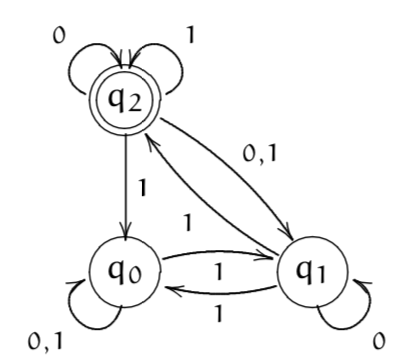
\includegraphics[width=5cm]{Fig1.png}
        \end{minipage}
        \item \begin{minipage}{\linewidth}
            \centering
            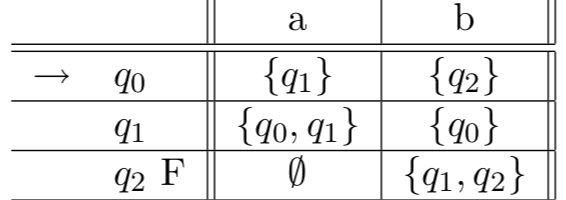
\includegraphics[width=5cm]{Fig2.png}
        \end{minipage}
    \end{itemize}
    \subsection{Soluzioni}
    DFA
    \begin{itemize}
        \item \begin{minipage}{\linewidth}
            \centering
            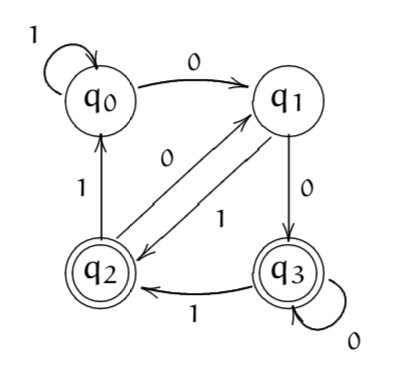
\includegraphics[width=5cm]{SolDFA1.png}
        \end{minipage}
        \item \begin{minipage}{\linewidth}
            \centering
            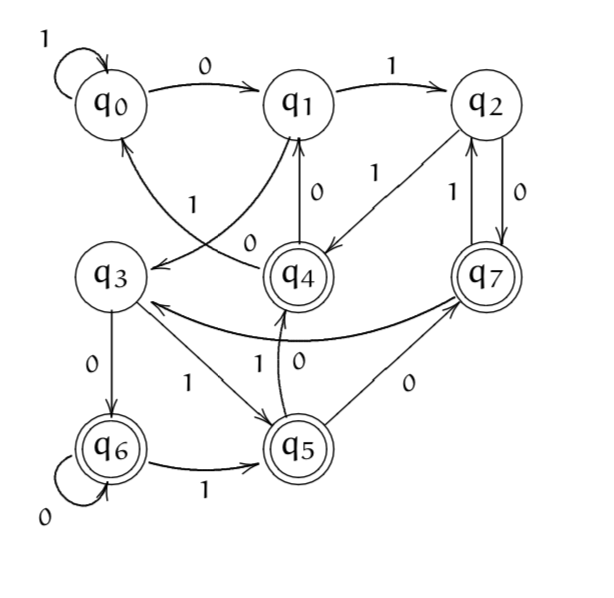
\includegraphics[width=5cm]{SolDFA2.png}
        \end{minipage}
        \item \begin{minipage}{\linewidth}
            \centering
            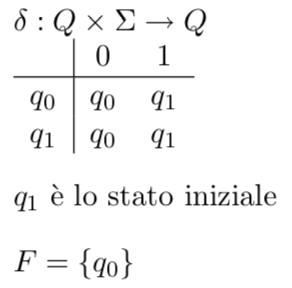
\includegraphics[width=5cm]{SolDFA4.png}
        \end{minipage}
        \item \begin{minipage}{\linewidth}
            \centering
            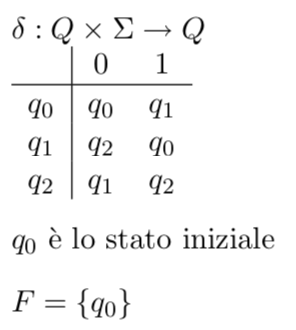
\includegraphics[width=5cm]{SolDFA3.png}
        \end{minipage}
    \end{itemize}
    NFA
    \begin{itemize}
        \item \begin{minipage}{\linewidth}
            \centering
            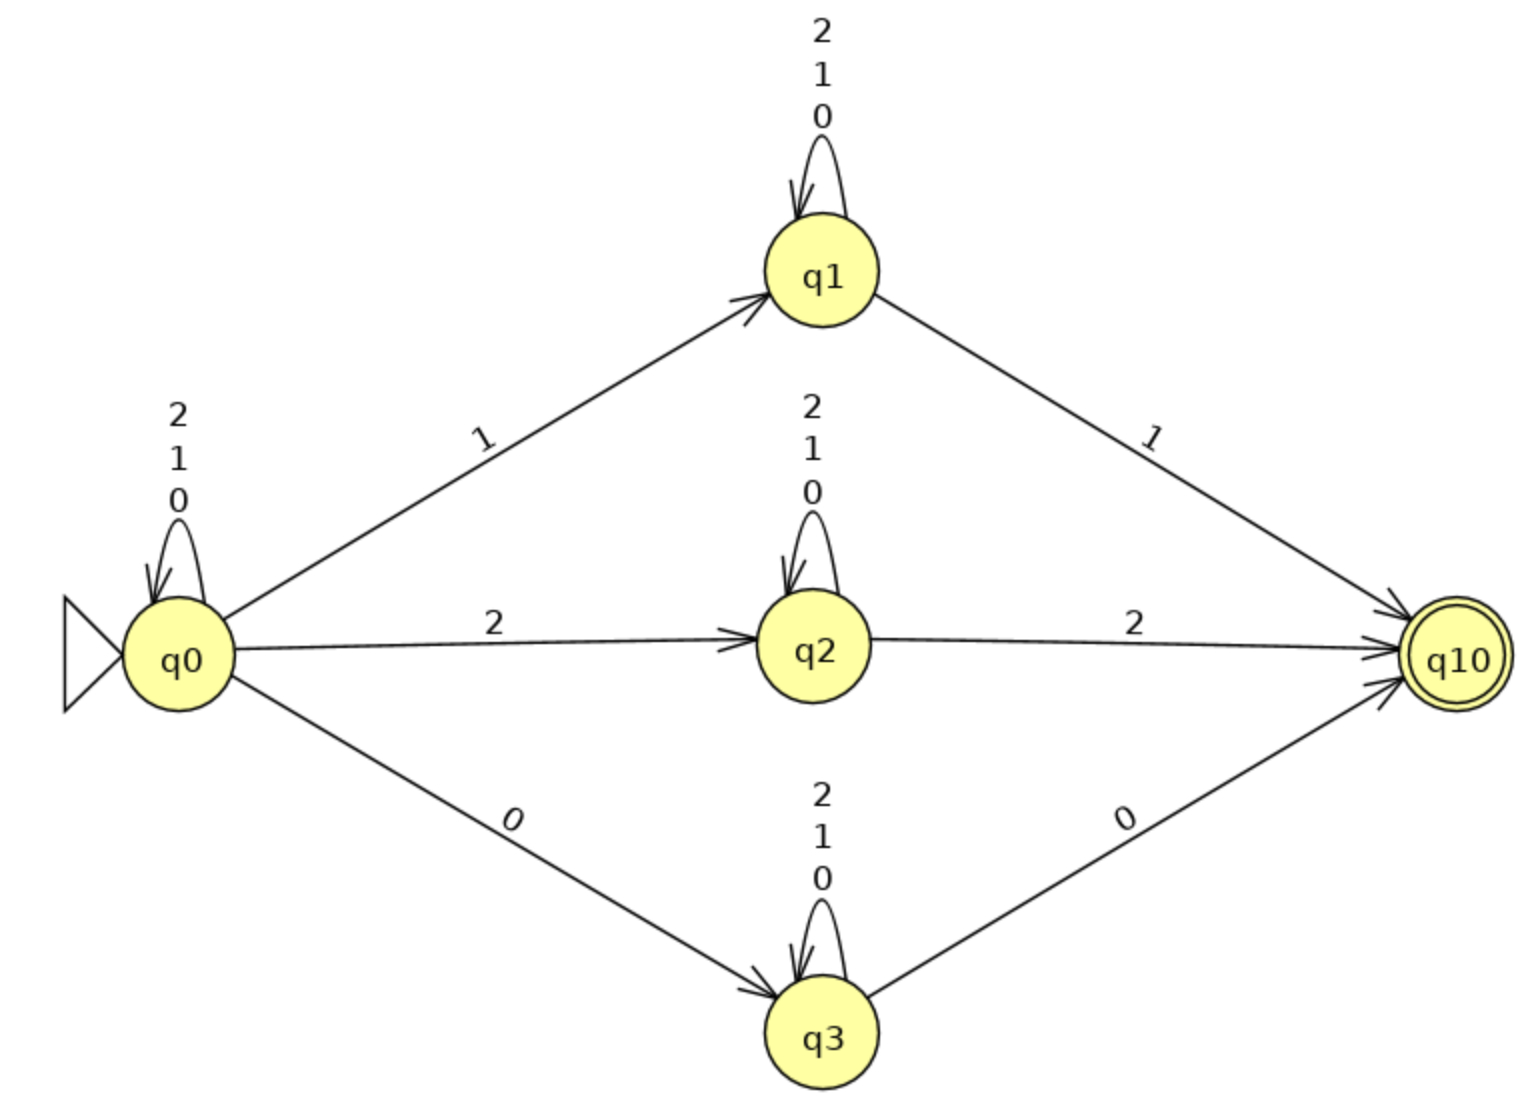
\includegraphics[width=5cm]{SolNFA2.png}
        \end{minipage}   
        \item \begin{minipage}{\linewidth}
            \centering
            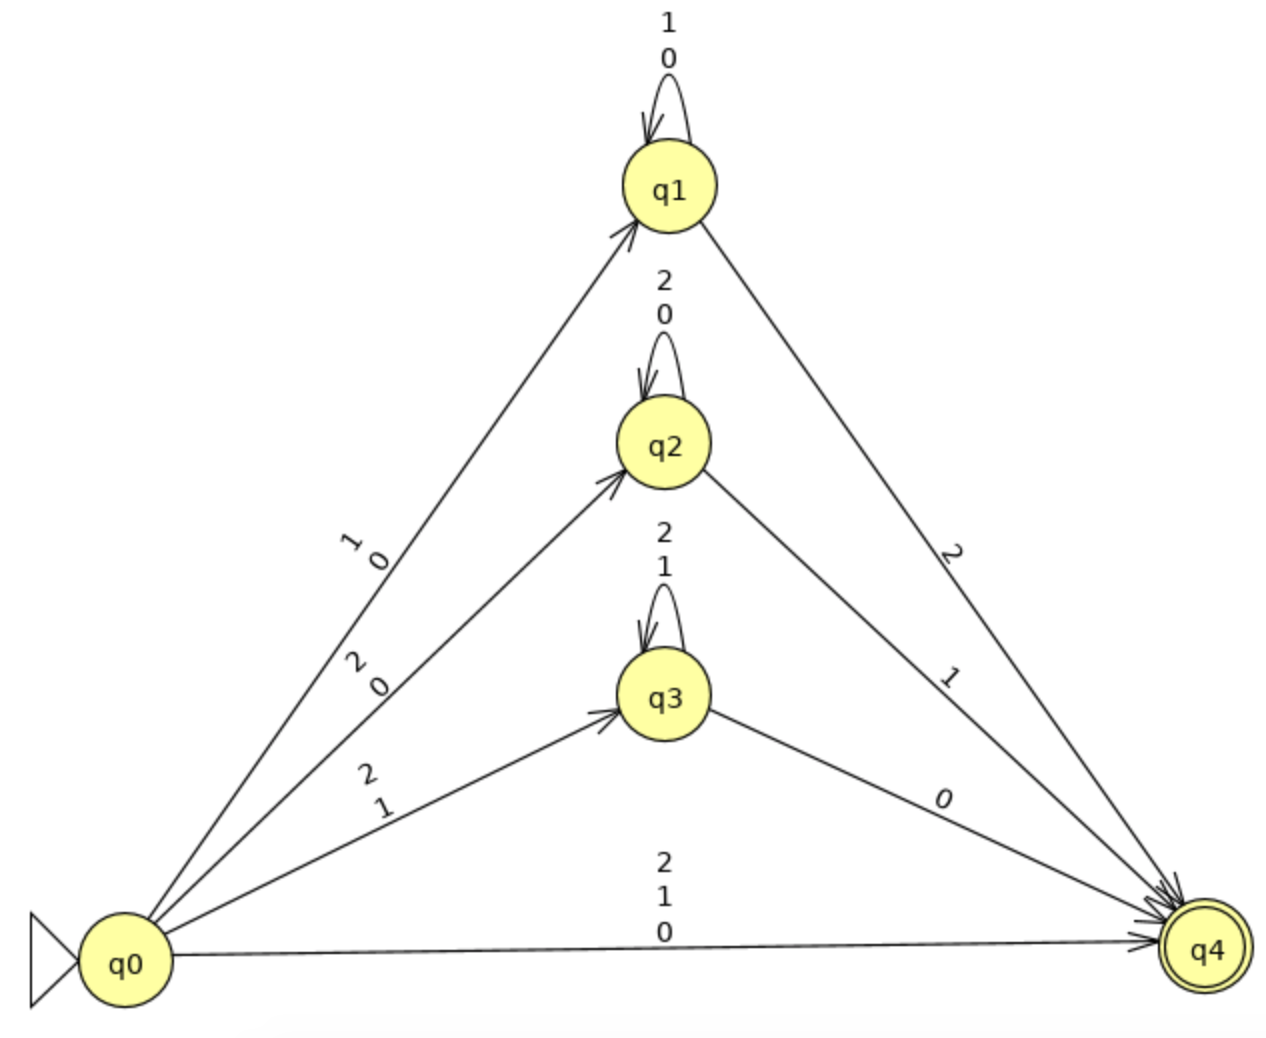
\includegraphics[width=5cm]{SolNFA3.png}
        \end{minipage}   
    \end{itemize}
    \begin{math}\epsilon
    \end{math}-NFA
    \begin{itemize}
        \item \begin{minipage}{\linewidth}
            \centering
            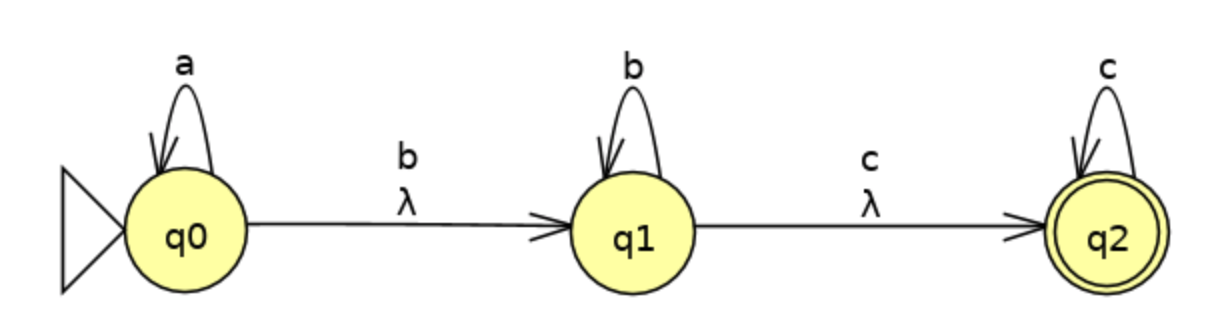
\includegraphics[width=5cm]{SolEPS1.png}
        \end{minipage}
        \item \begin{minipage}{\linewidth}
            \centering
            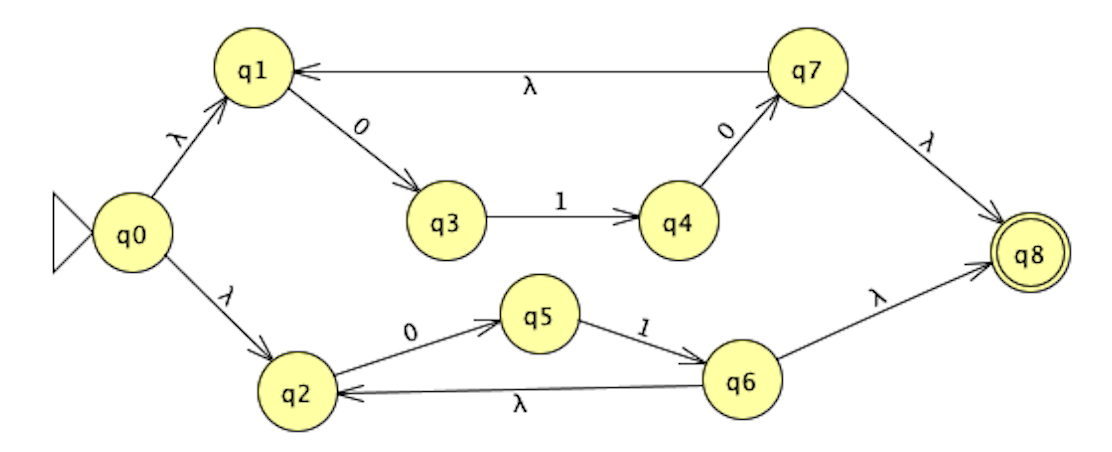
\includegraphics[width=5cm]{SolEPS2.png}
        \end{minipage}  
        \item \begin{minipage}{\linewidth}
            \centering
            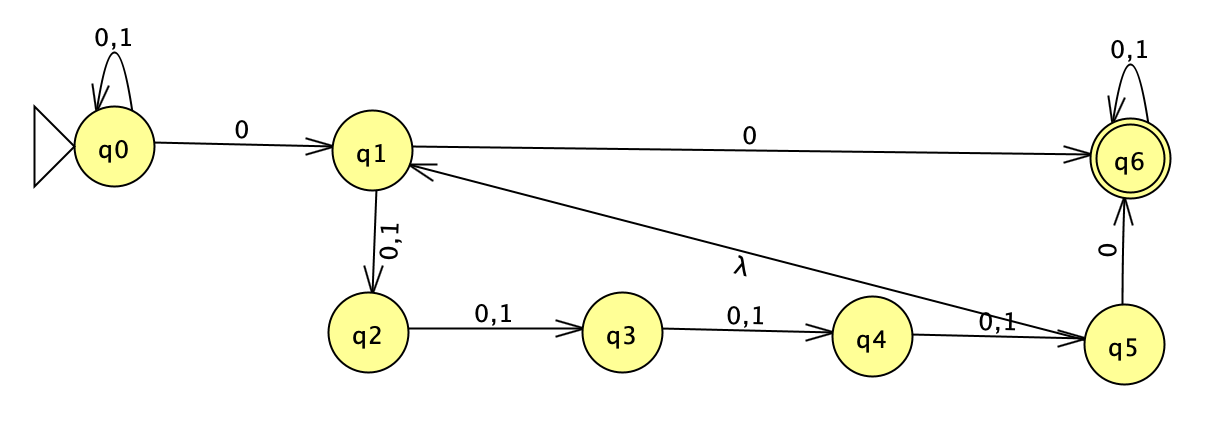
\includegraphics[width=5cm]{SolEPS3.png}
        \end{minipage}  
    \end{itemize}
    % Bibliografia
    %\begin{thebibliography}{9}
        %  Alcune soluzio
    %\end{thebibliography}
    \end{document}